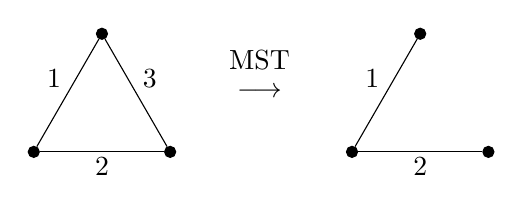
\begin{tikzpicture}[black/.style={circle,draw,fill=black,inner sep=0pt, minimum width=4pt}]
	\foreach \x in {90,210,330}
		\node[black] at (\x:1) (\x) {};
	\draw (90) -- (210) node [midway,label={1},xshift=-5,yshift=-5] {};
	\draw (210) -- (330) node [midway,label=below:{2},yshift=5] {};
	\draw (330) -- (90) node [midway,label={3},xshift=5,yshift=-5] {};


	\draw node at (2,0.25) {$\longrightarrow$};
	\draw[above,yshift=5] node at (2,0.25) {MST};


	\foreach \x in {90,210,330}
		\node[black,xshift=115] at (\x:1) (\x) {};
	\draw (90) -- (210) node [midway,label={1},xshift=-5,yshift=-5] {};
	\draw (210) -- (330) node [midway,label=below:{2},yshift=5] {};
	% \draw (330) -- (90) node [midway,label={3},xshift=5,yshift=-5] {};
\end{tikzpicture}
